\documentclass[11pt]{article}
\usepackage[a4paper,margin=2cm]{geometry}
\usepackage{graphicx,booktabs,amsmath,float,caption}
\usepackage[hidelinks]{hyperref}
\setlength{\parskip}{4pt}\setlength{\parindent}{0pt}

\title{\textbf{PRML Lab 2 --- Decision Trees}}
\author{Aryan Tiwari (B20AI056)\\CSL2050 Pattern Recognition \& Machine Learning, Winter 2022}
\date{}

\begin{document}
\maketitle

\section*{Question 1 --- Classification tree from scratch (Penguins)}

\textbf{Cost function.} My roll number (56) is even, so every split is chosen with \textbf{entropy},
$H(S)=-\sum_c p_c\log_2 p_c$, and the quality of a split is its information gain
$IG = H(\text{parent}) - \sum_k \frac{|S_k|}{|S|}H(S_k)$.
The training labels have $H=1.513$ bits (the maximum for 3 classes is $\log_2 3=1.585$).

\textbf{Pre-processing.} Two rows had no measurements at all and were dropped. \texttt{sex} was missing for
9 more rows and was filled with the mode. \texttt{year} only records when the bird was observed, so it was
dropped to stop the tree from learning a rule that has nothing to do with the species. \texttt{island} and \texttt{sex}
are nominal and label-encoded; the tree splits multi-way on them, so the codes carry no order.
The 342 remaining samples were split 80:20 (273 train / 69 test), stratified by species.

\begin{figure}[H]\centering
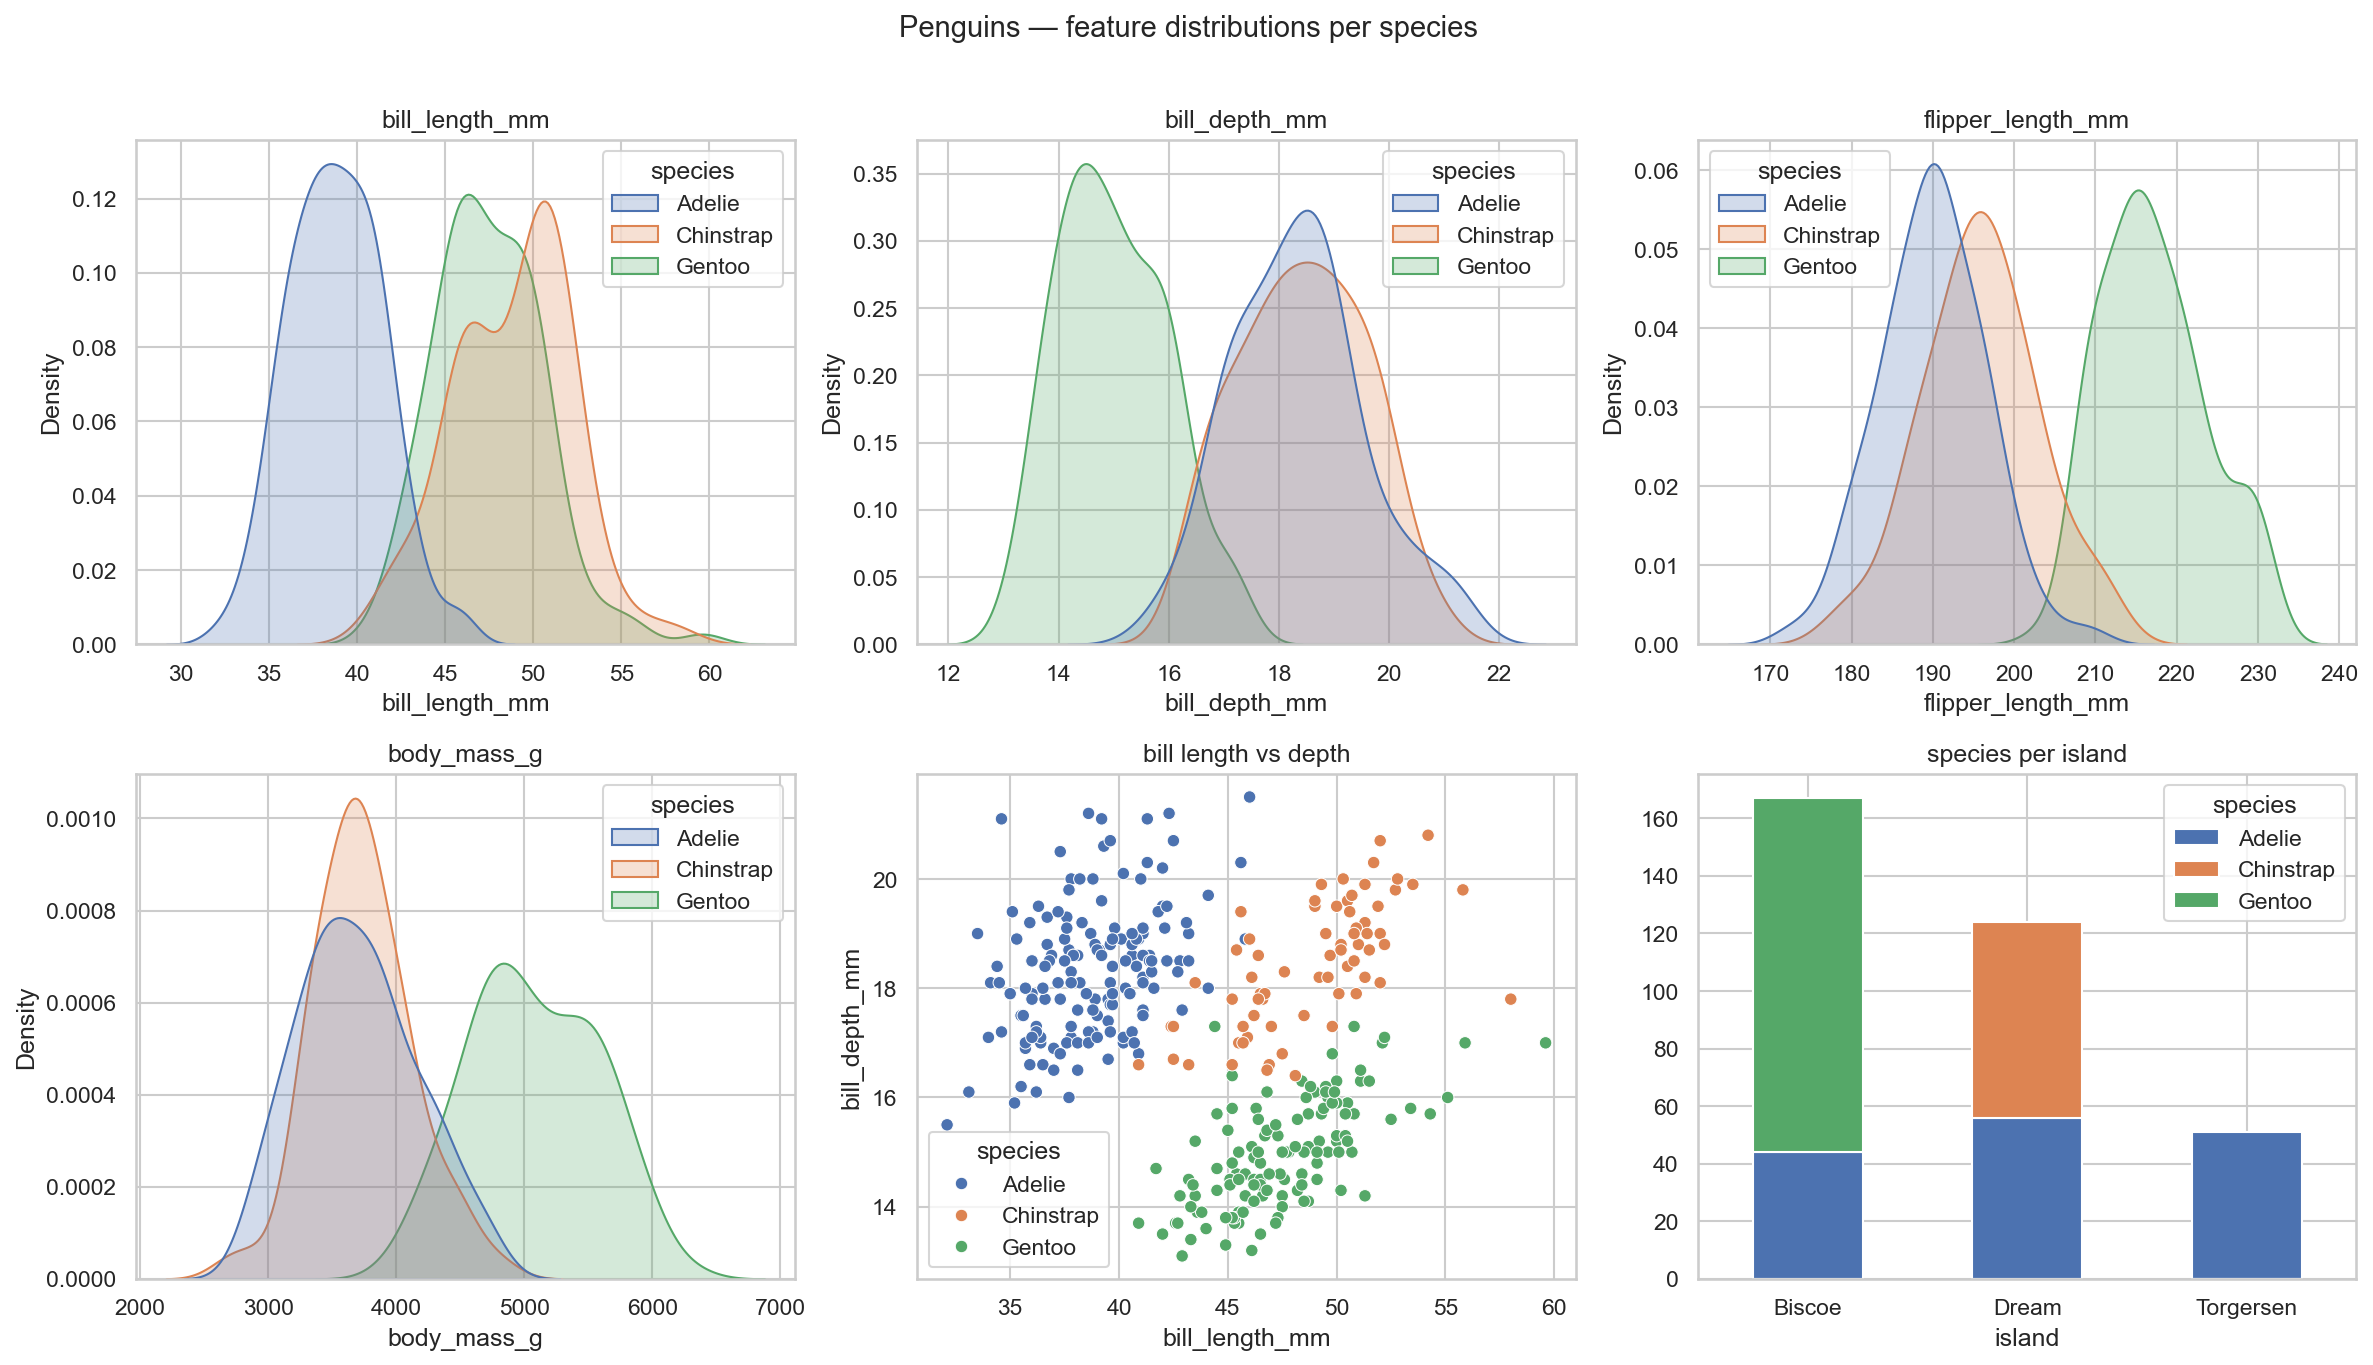
\includegraphics[width=\linewidth]{figures/q1_eda.png}
\caption{Per-species distributions. Flipper length and body mass isolate Gentoo; bill length separates Adelie
from Chinstrap; Chinstrap is only found on Dream and Gentoo only on Biscoe.}
\end{figure}

\textbf{\texttt{cont\_to\_cat()}.} Each continuous feature is binarised independently. Candidate thresholds are
midpoints between consecutive distinct values, and the one with the lowest weighted child entropy is kept.
Thresholds are learnt on the training set and reused unchanged on the test set.

\begin{table}[H]\centering
\begin{tabular}{lcc}\toprule
Feature & Threshold & Information gain (bits)\\\midrule
bill\_length\_mm & 42.35 & 0.791\\
bill\_depth\_mm & 16.35 & 0.692\\
flipper\_length\_mm & 207.5 & 0.797\\
body\_mass\_g & 4362.5 & 0.582\\\bottomrule
\end{tabular}
\caption{Learnt binarisation thresholds.}
\end{table}

\textbf{Training.} The tree is grown ID3-style: at each node the attribute with the highest information gain
is chosen, one child is created per value, and the procedure recurses with that attribute removed.
Growth stops when (i) the node reaches \texttt{max\_depth}, (ii) the best attainable gain is $\le 10^{-6}$
(no information gain --- the model has plateaued), (iii) the node is pure, or (iv) no attributes remain.
Each node stores its majority class, which is the prediction at a leaf and the fallback when a test sample
has an attribute value never seen during training. The root split is \texttt{flipper\_length} (largest gain).

\begin{table}[H]\centering
\begin{tabular}{cccc}\toprule
\texttt{max\_depth} & Learnt depth & Train acc. & Test acc.\\\midrule
1 & 1 & 0.791 & 0.783\\
2 & 2 & 0.971 & 0.899\\
3 & 3 & 0.989 & 0.957\\
4 & 4 & 0.993 & 0.986\\
5 & 5 & 0.993 & 0.986\\
6 & 5 & 0.993 & 0.986\\\bottomrule
\end{tabular}
\caption{Effect of the depth limit. From depth 5 onwards the tree stops by itself because no split adds information.}
\end{table}

\textbf{Results.} With \texttt{max\_depth}=5 the test accuracy is \textbf{98.55\%} (68/69).
Class-wise: Adelie 100\% (30/30), Chinstrap 92.86\% (13/14), Gentoo 100\% (25/25). The single error is a
Chinstrap predicted as Adelie --- the two species overlap in bill depth, flipper length and mass, and differ
mainly in bill length, which binarisation reduces to a single cut. Train accuracy stays at 99.3\% rather than
100\% for the same reason: once features are binarised, a few samples from different classes become identical.

\section*{Question 2 --- Regression tree (Energy Efficiency, heating load $Y_1$)}

\textbf{Pre-processing.} 768 samples, 8 numeric features, no missing values or duplicates. Trees split on
thresholds, so they don't need feature scaling; the integer-coded features (orientation X6, glazing distribution X8)
are used as they are. The data was split 70:10:20 into train (537), validation (77) and test (154) sets.

\textbf{Hyper-parameters varied (manual loops, no grid-search utilities).}
\begin{itemize}\itemsep0pt
\item \texttt{max\_depth} --- the main capacity control. Shallow trees underfit (high bias); deep trees can memorise noise.
\item \texttt{min\_samples\_leaf} --- every prediction averages at least this many samples; larger values smooth the fit and reduce variance.
\item \texttt{min\_samples\_split} --- a node needs this many samples before it may split; another brake on growth.
\end{itemize}

\begin{figure}[H]\centering
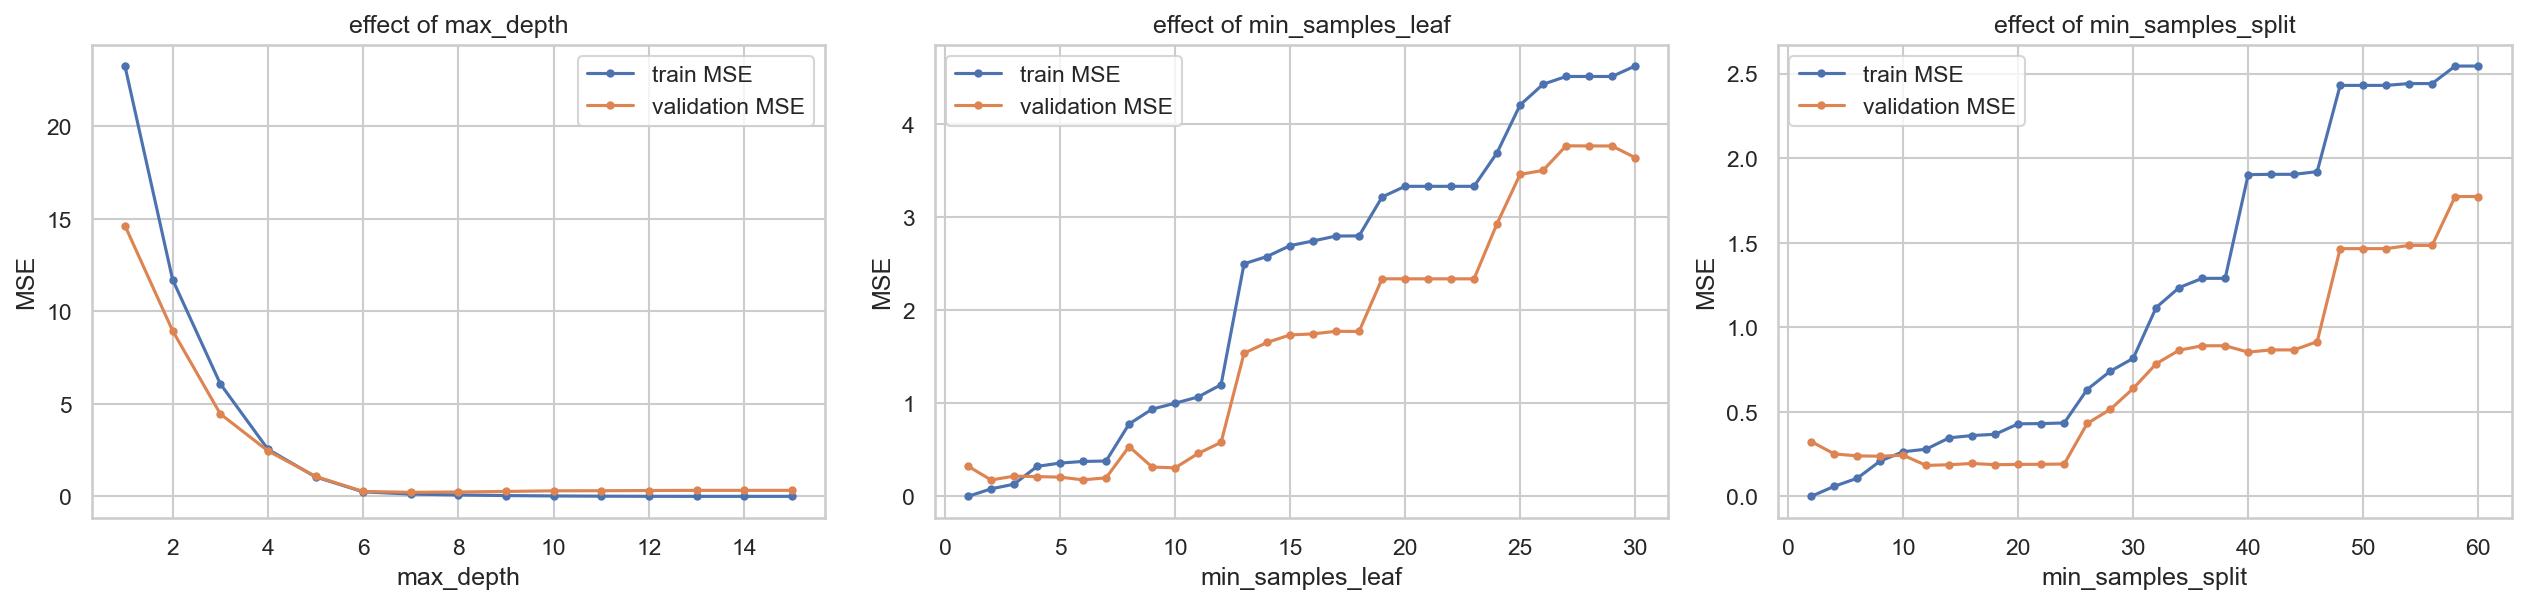
\includegraphics[width=\linewidth]{figures/q2_sweeps.png}
\caption{Train and validation MSE when each hyper-parameter is varied on its own.}
\end{figure}

Validation MSE drops steeply up to depth $\approx 6$ and then flattens: the heating load is almost a
deterministic function of the building geometry, so extra depth adds little and costs little. Raising
\texttt{min\_samples\_leaf} or \texttt{min\_samples\_split} raises \emph{both} curves in steps, which
means it underfits rather than regularises: there is very little noise for these constraints to remove. A joint search over
$14\times6\times4=336$ combinations selected \texttt{max\_depth}=9, \texttt{min\_samples\_leaf}=2,
\texttt{min\_samples\_split}=2 with validation MSE \textbf{0.175}.

\begin{figure}[H]\centering
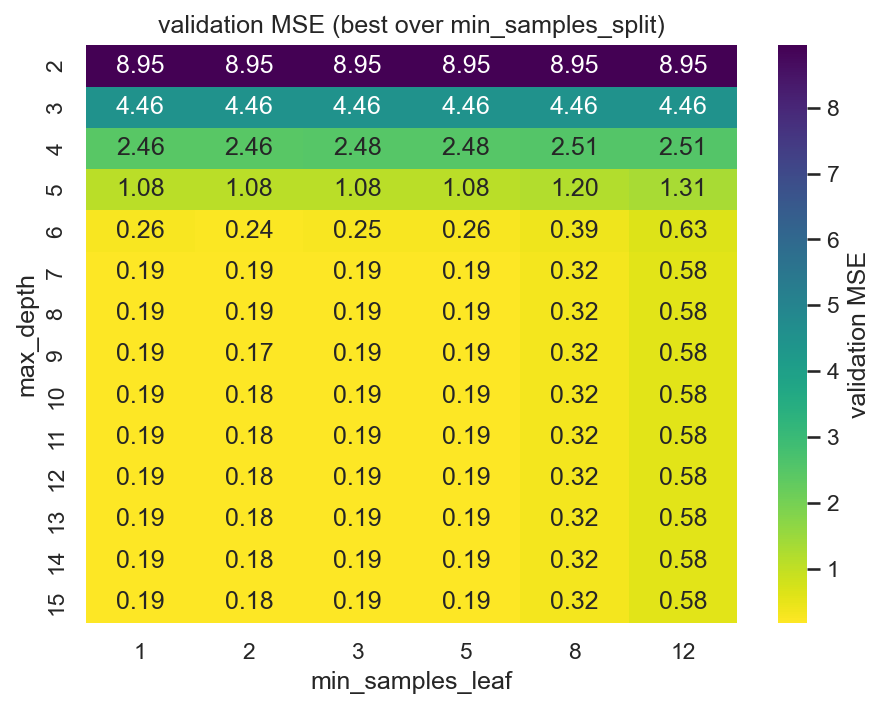
\includegraphics[width=0.55\linewidth]{figures/q2_heatmap.png}
\caption{Validation MSE over depth $\times$ minimum leaf size.}
\end{figure}

\textbf{5-fold cross-validation and test.} With the chosen hyper-parameters, 5-fold CV on the
train+validation data gives fold MSEs of 0.226, 0.771, 0.277, 0.297, 0.288 --- mean
\textbf{0.372 $\pm$ 0.201}. Fold 2 is about three times worse than the others, so the error depends
noticeably on which buildings end up in the held-out fold; the mean over folds is a fairer estimate than any
single validation split. The final tree, refit on all train+validation data, gets a \textbf{test MSE of 0.328}
(RMSE 0.57 on a target ranging 6.0--43.1). It is 9 levels deep with 219 leaves.

\begin{figure}[H]\centering
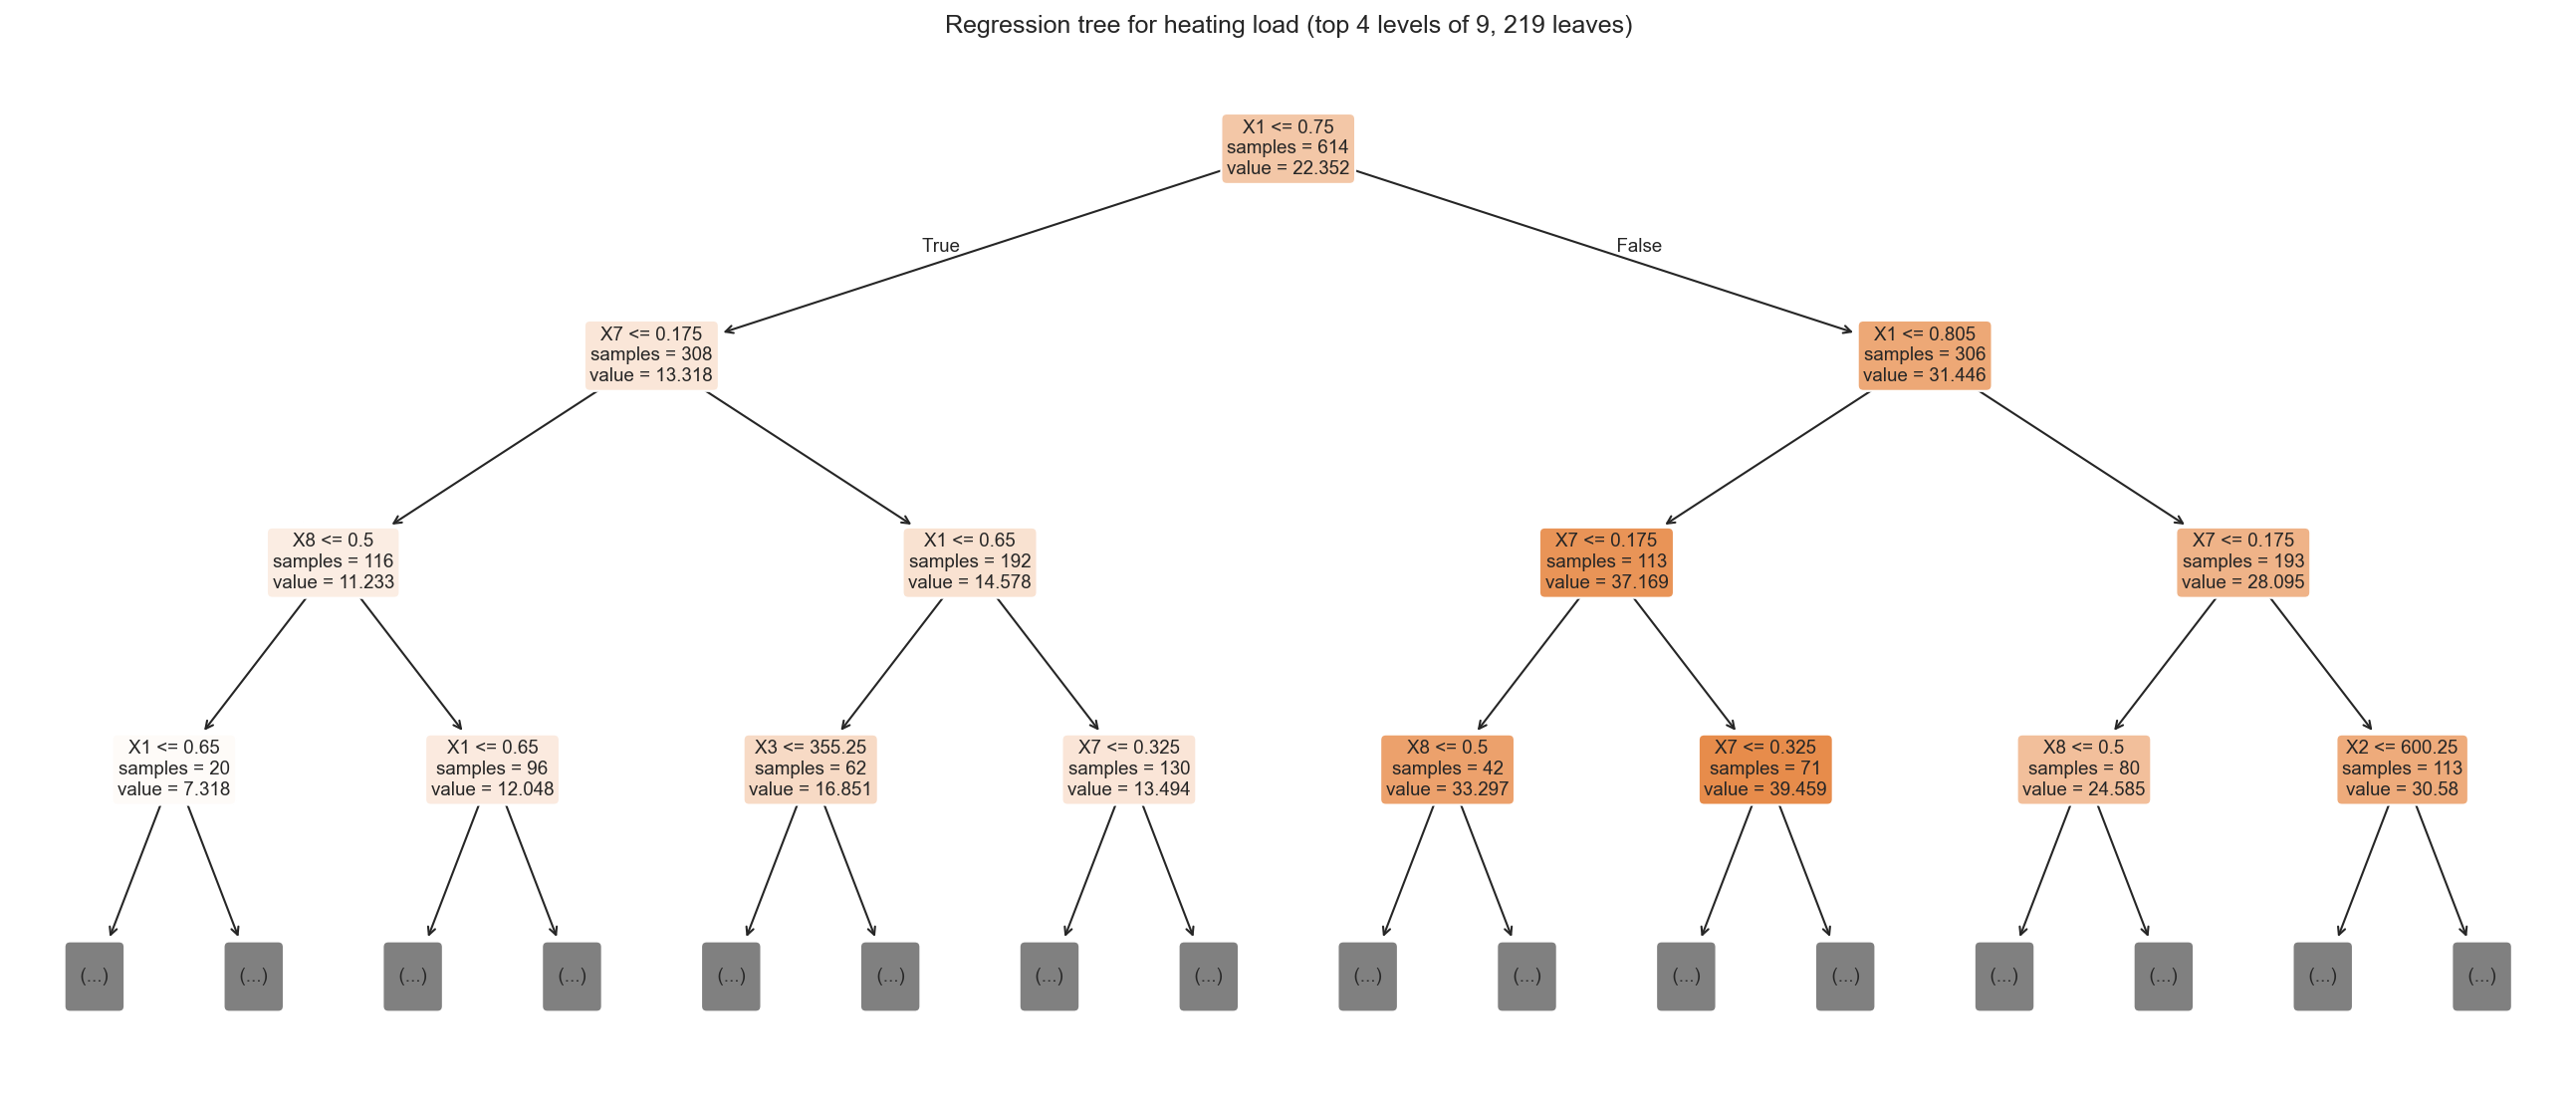
\includegraphics[width=\linewidth]{figures/q2_tree.png}
\caption{Top four levels of the final regression tree.}
\end{figure}

Feature importances show that relative compactness (X1) accounts for 89.7\% of the impurity reduction, followed by glazing
area X7 (6.5\%) and its distribution X8 (2.2\%). Compactness controls how much surface area loses heat, so
this agrees with the physics.

\end{document}
